\documentclass{beamer}

\usepackage{color} % Package to include colors for syntax highlighting
\usepackage{graphicx}  % Package to include images
\usepackage{hyperref}  % Hyperlinks
\usepackage{tikz}

\setbeamertemplate{navigation symbols}{}  % Remove navigation symbols
\usecolortheme[light]{solarized}

\title{Mid module feedback}
\date{}


\begin{document}

\frame{
    \titlepage
}

\frame{
    \begin{center}
        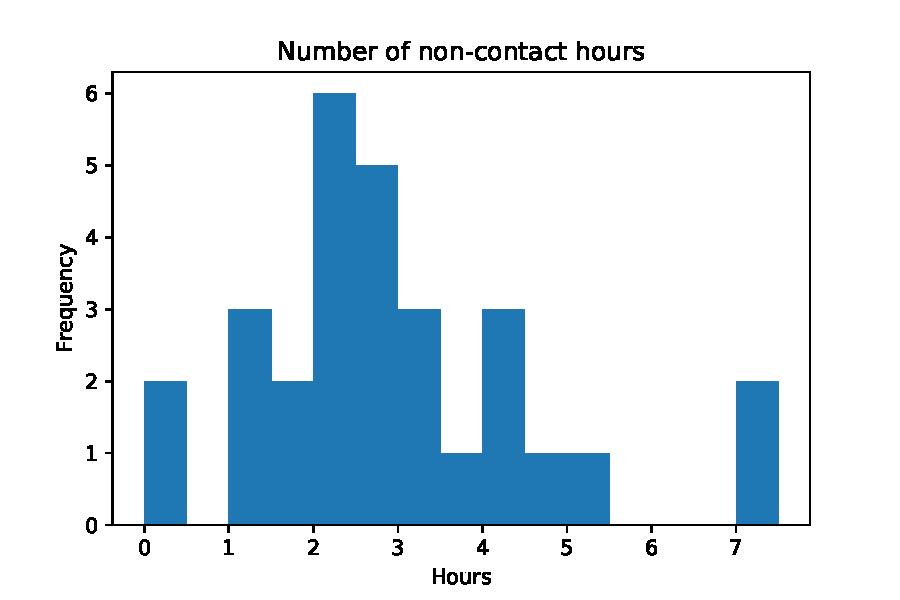
\includegraphics[width=.8\textwidth]{plot.pdf}
    \end{center}
}

\frame{
    \Large
    \begin{quote}
        Class site is good.
    \end{quote}
}

\frame{
    \Large
    \begin{quote}
    Working at my own pace is good
    \end{quote}
}

\frame{
    \Large
    \begin{quote}
        Like the class meetings.
    \end{quote}
}

\frame{
    \Large
    \begin{quote}
        ``Weirdly much more approachable than first year. (Very good thing).''
    \end{quote}
    \pause
    \begin{quote}
        ``Spending the first 20 minutes trying to convince everyone that you're
        not terrifying is slightly counter-productive''
    \end{quote}
}

\frame{
    \Large
    \begin{quote}
        ``Please bring your dog again.''
    \end{quote}
}

\frame{
    \begin{center}
        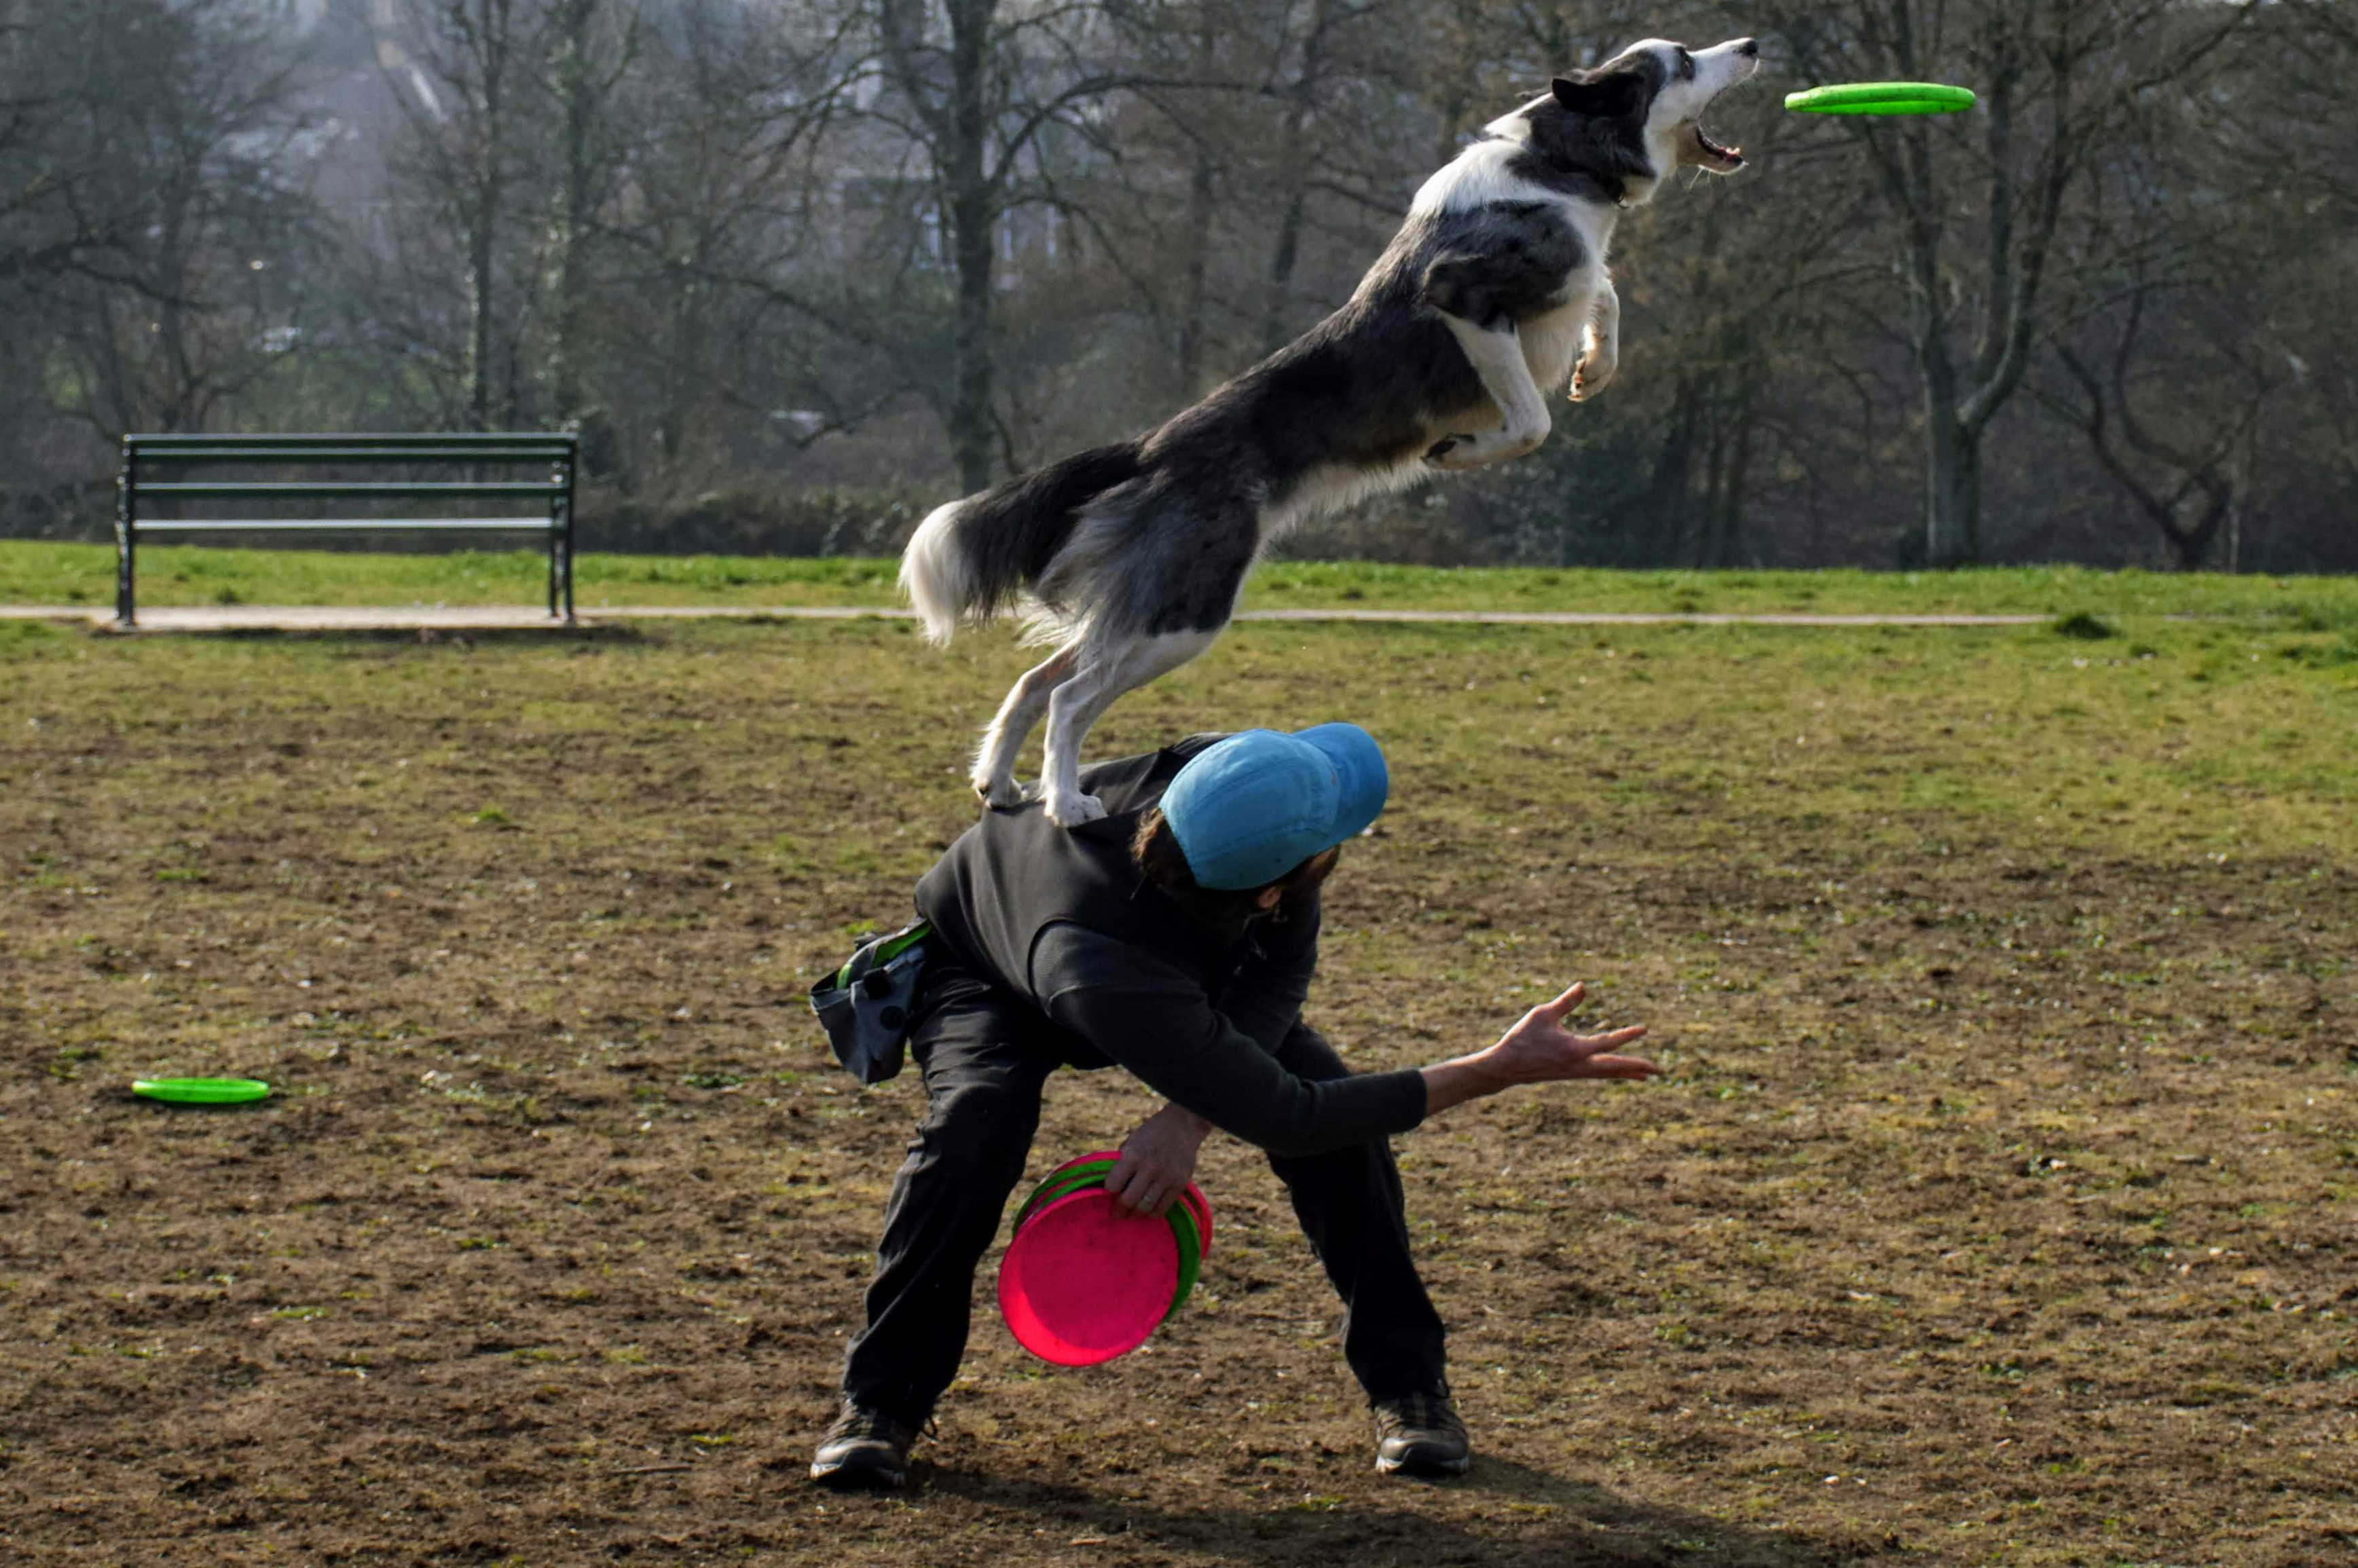
\includegraphics[width=.45\textwidth]{pup_1.jpg}
        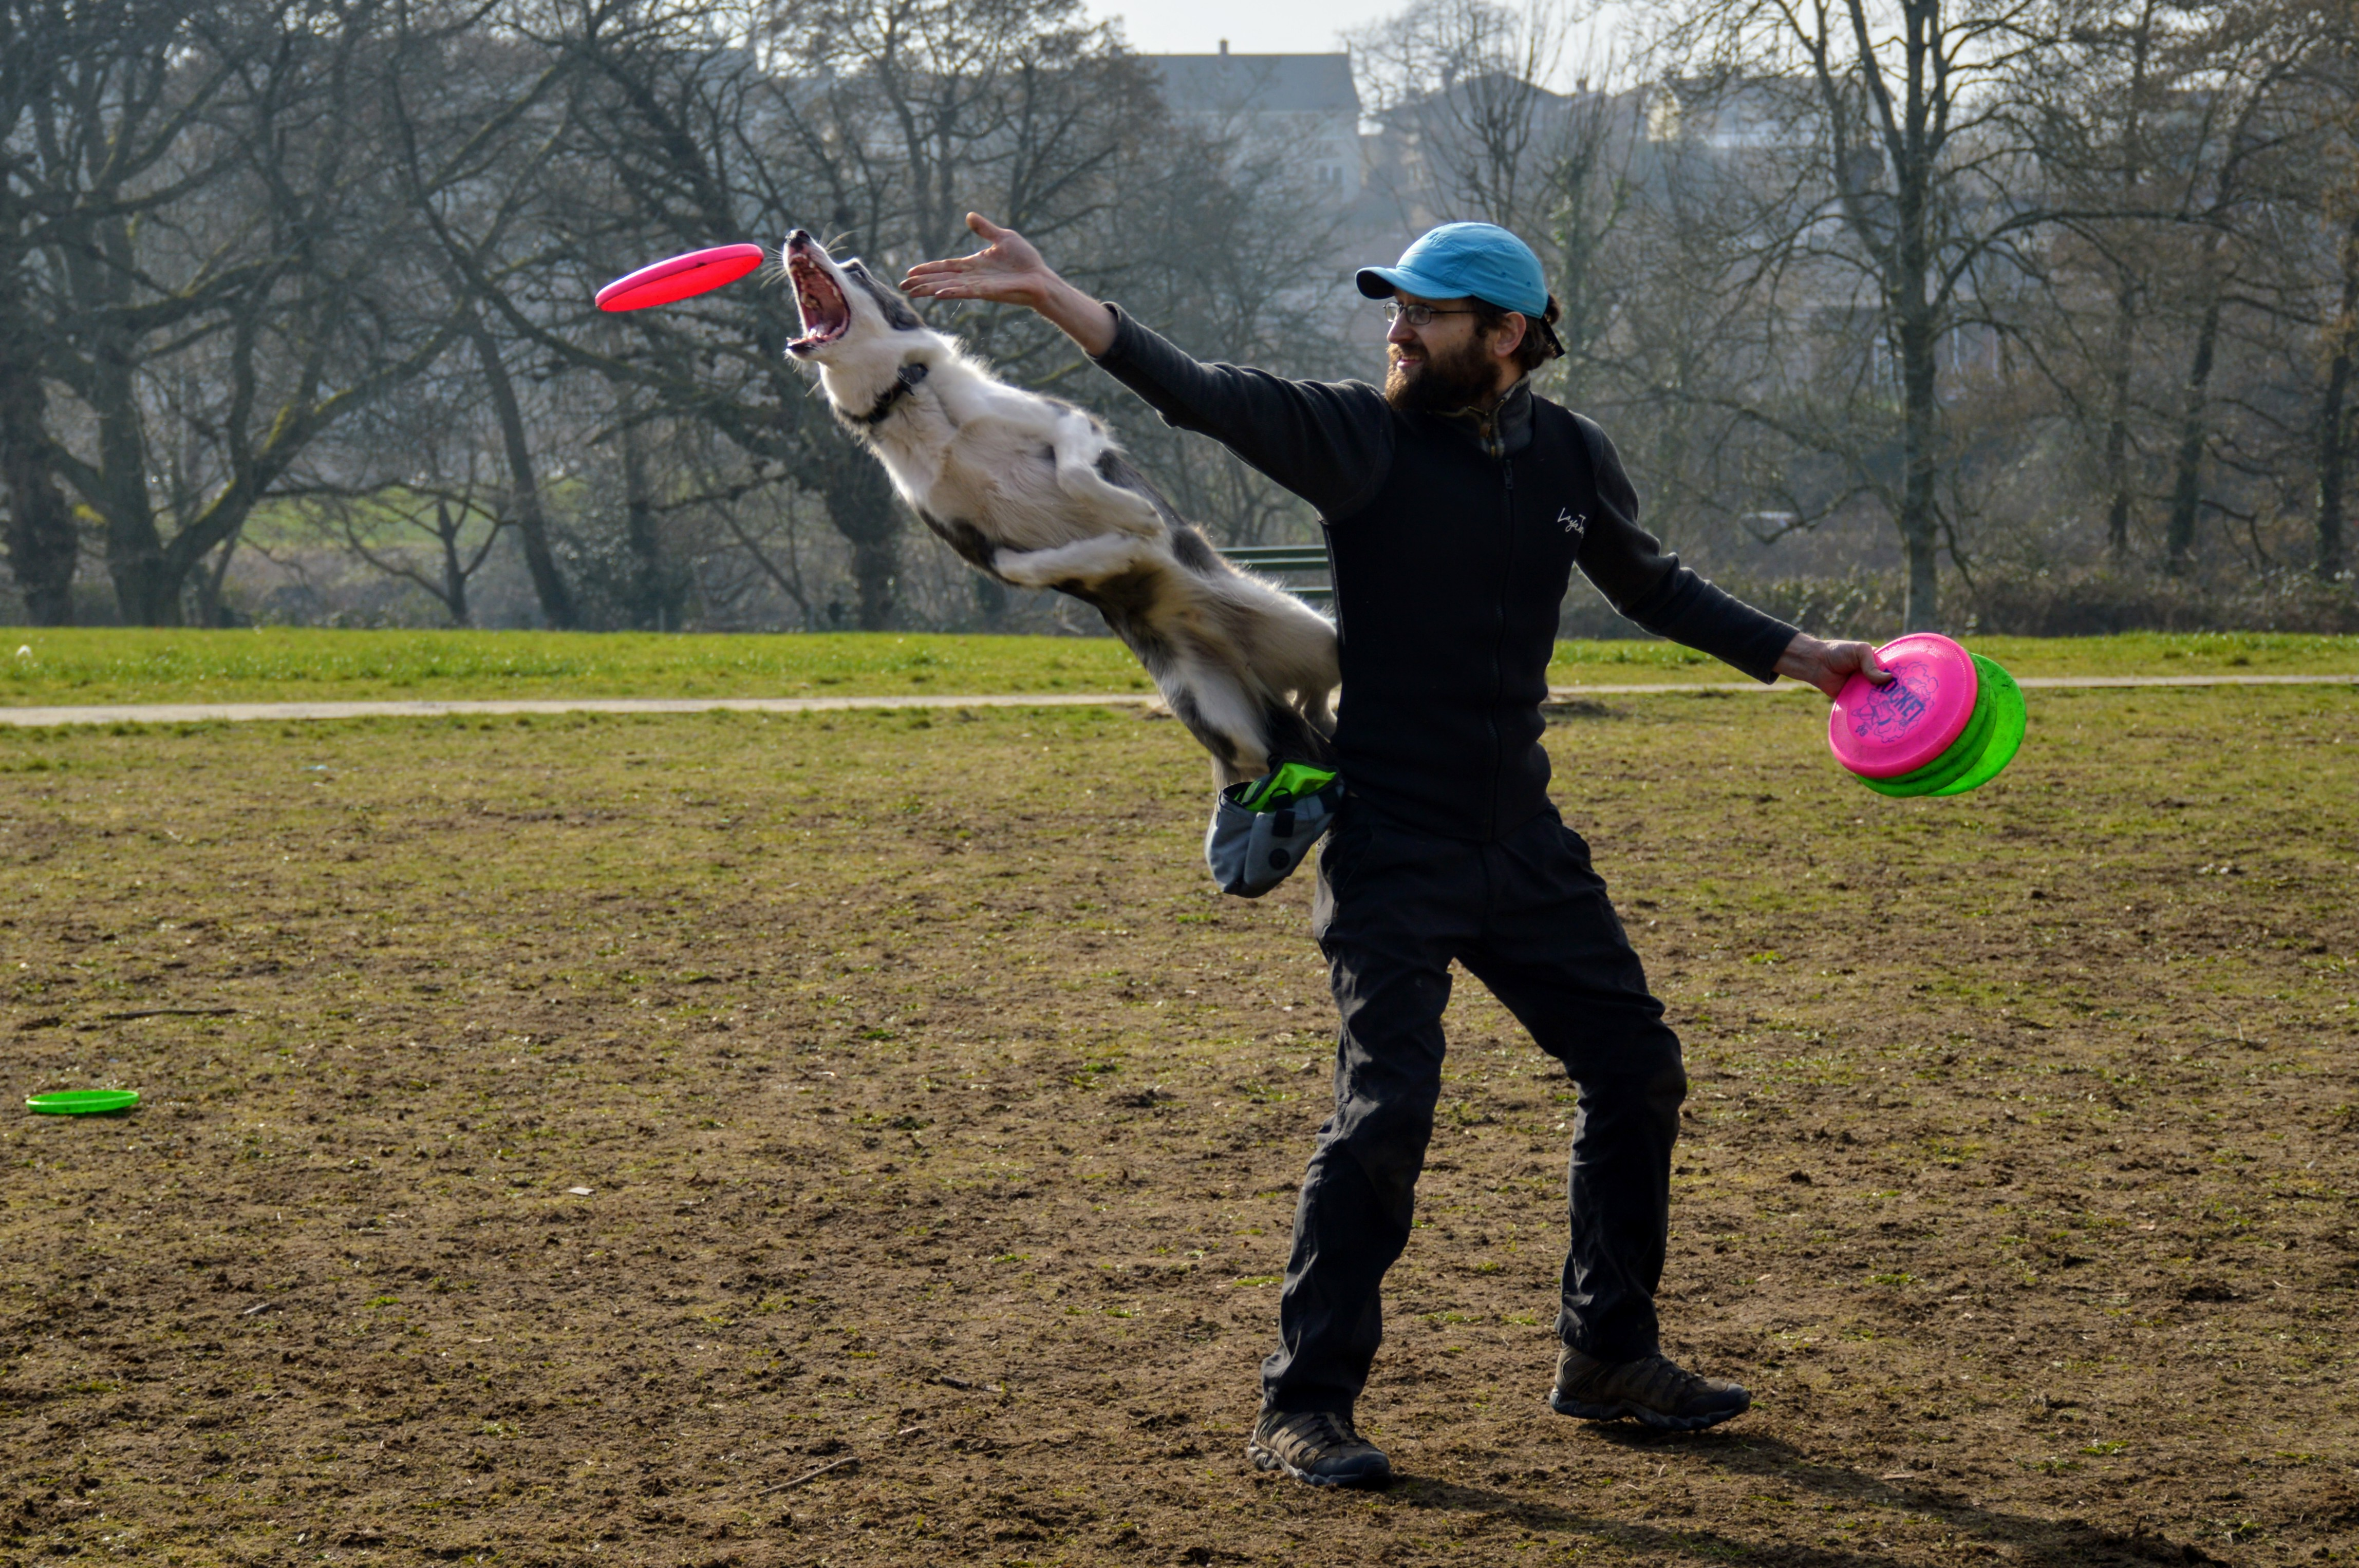
\includegraphics[width=.45\textwidth]{pup_2.jpg}

        \vspace{1cm}
        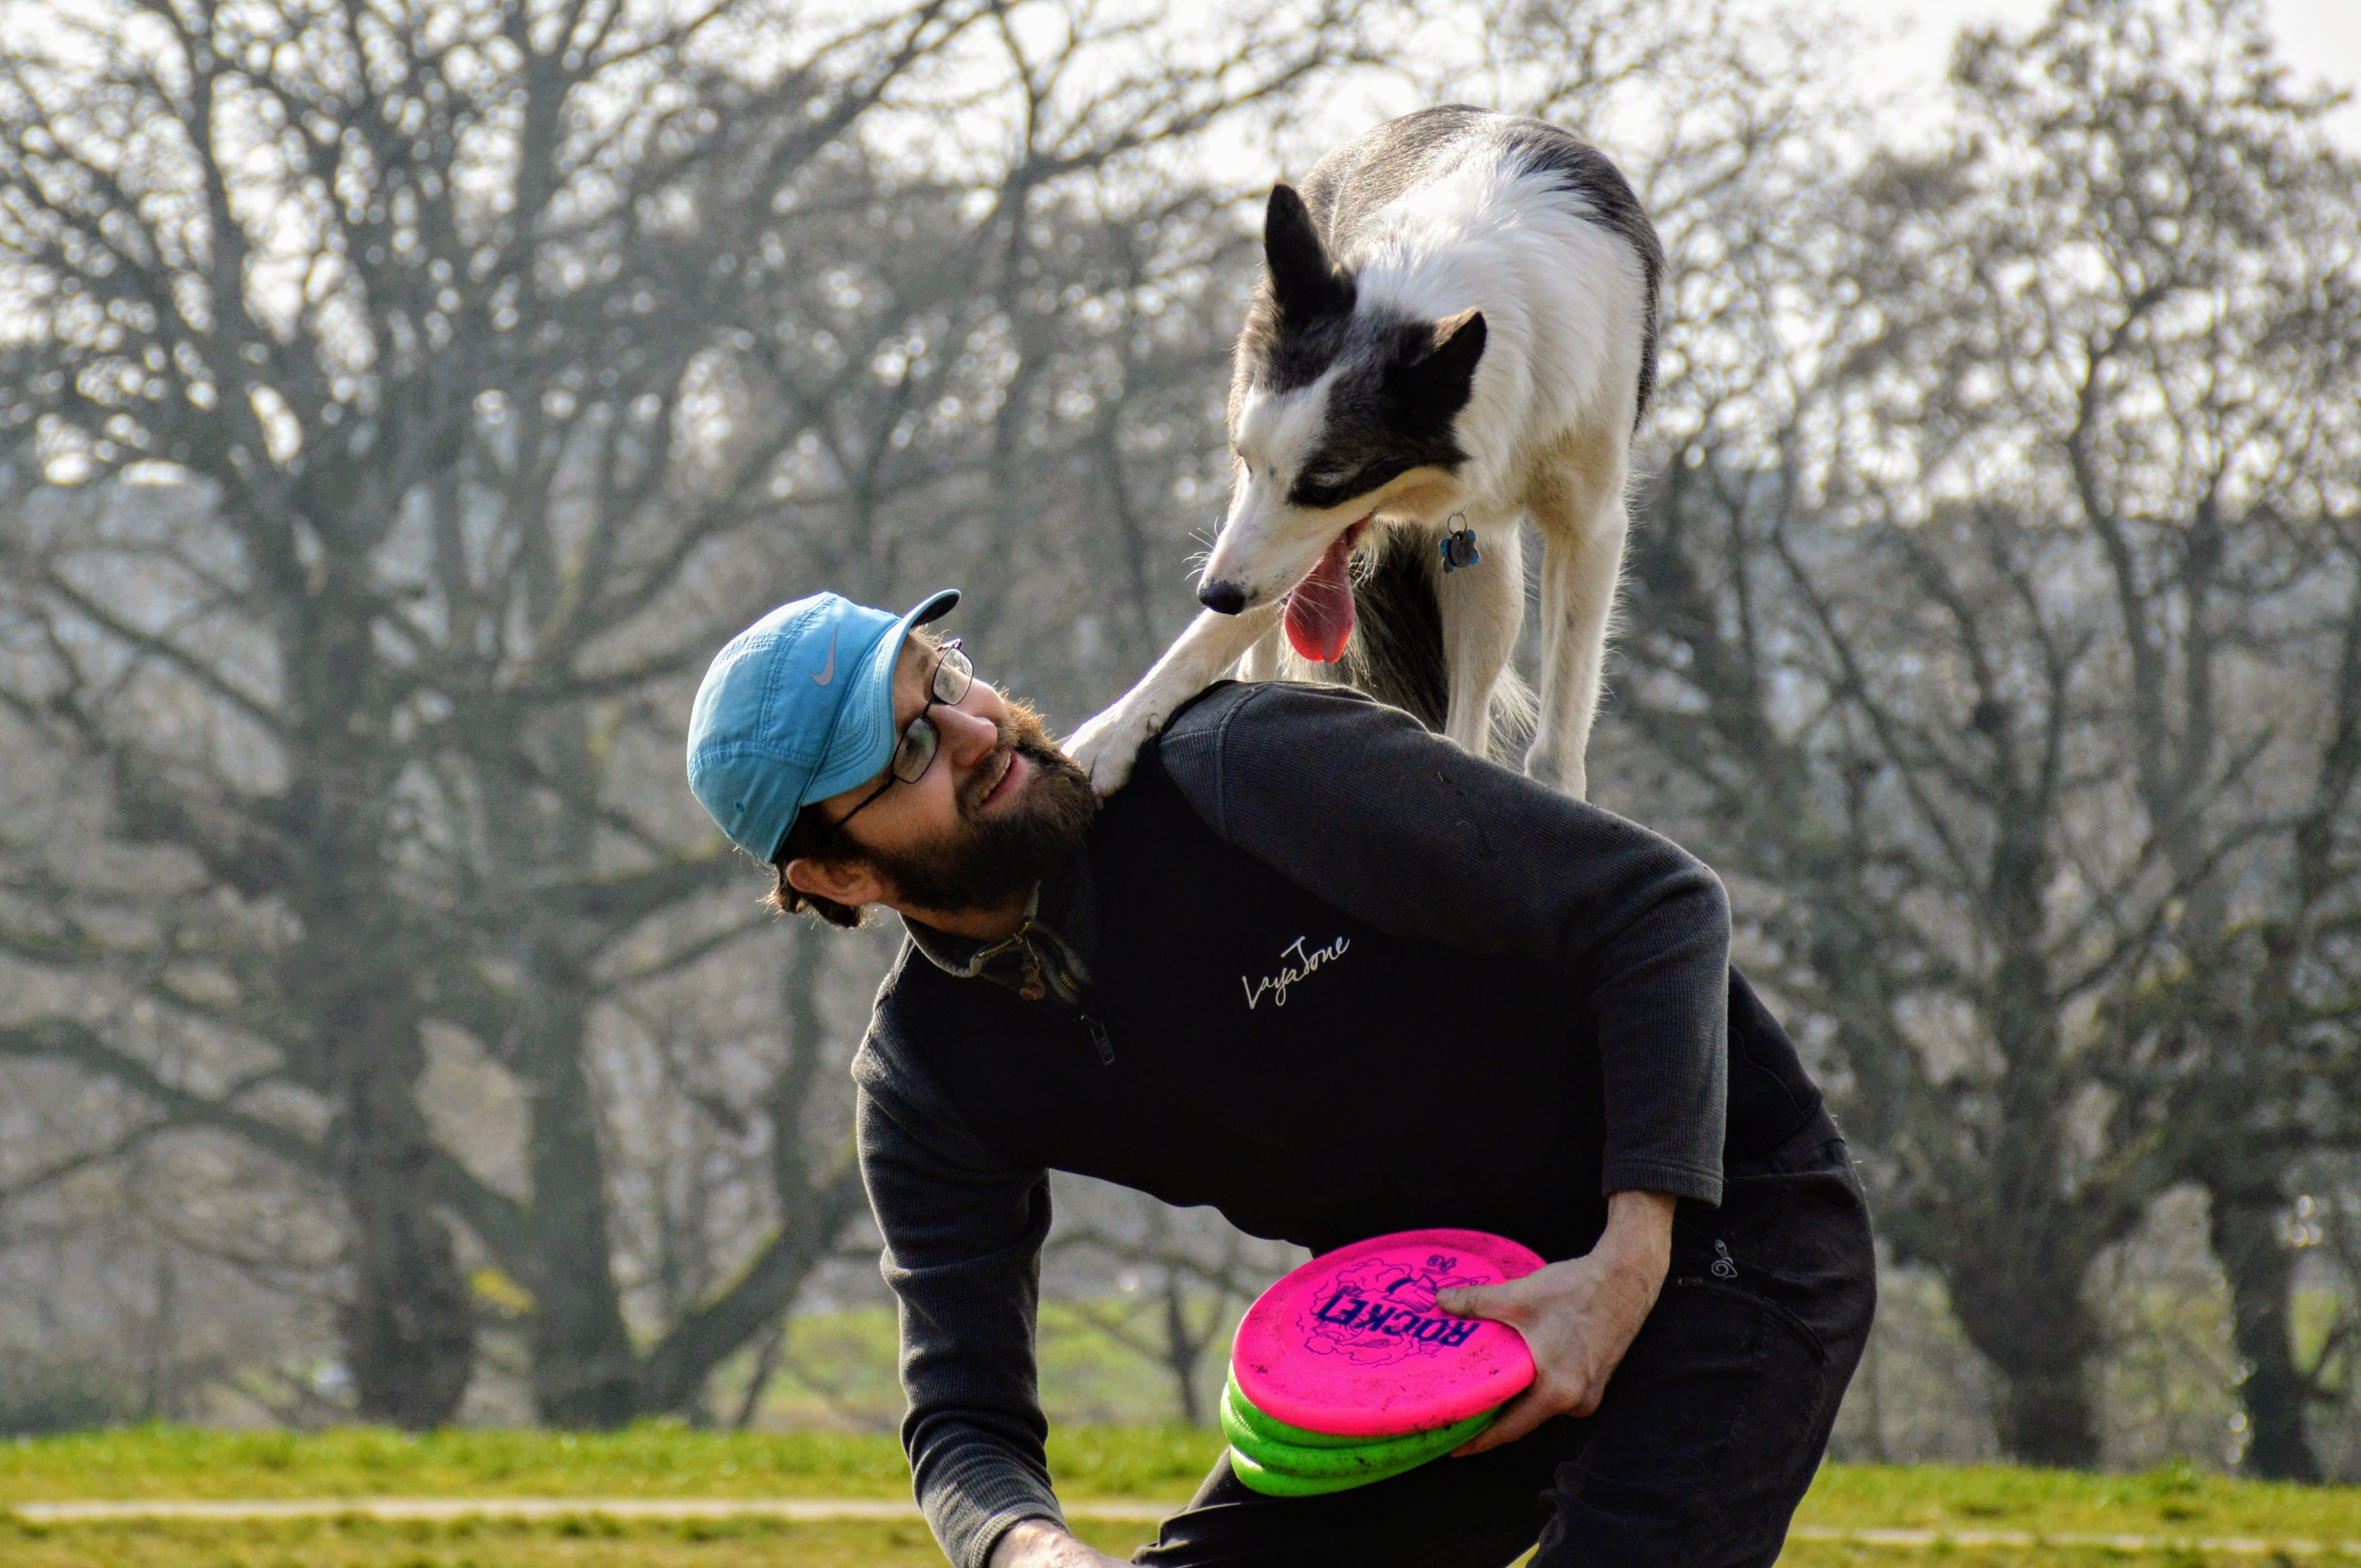
\includegraphics[width=.45\textwidth]{pup_3.jpg}
        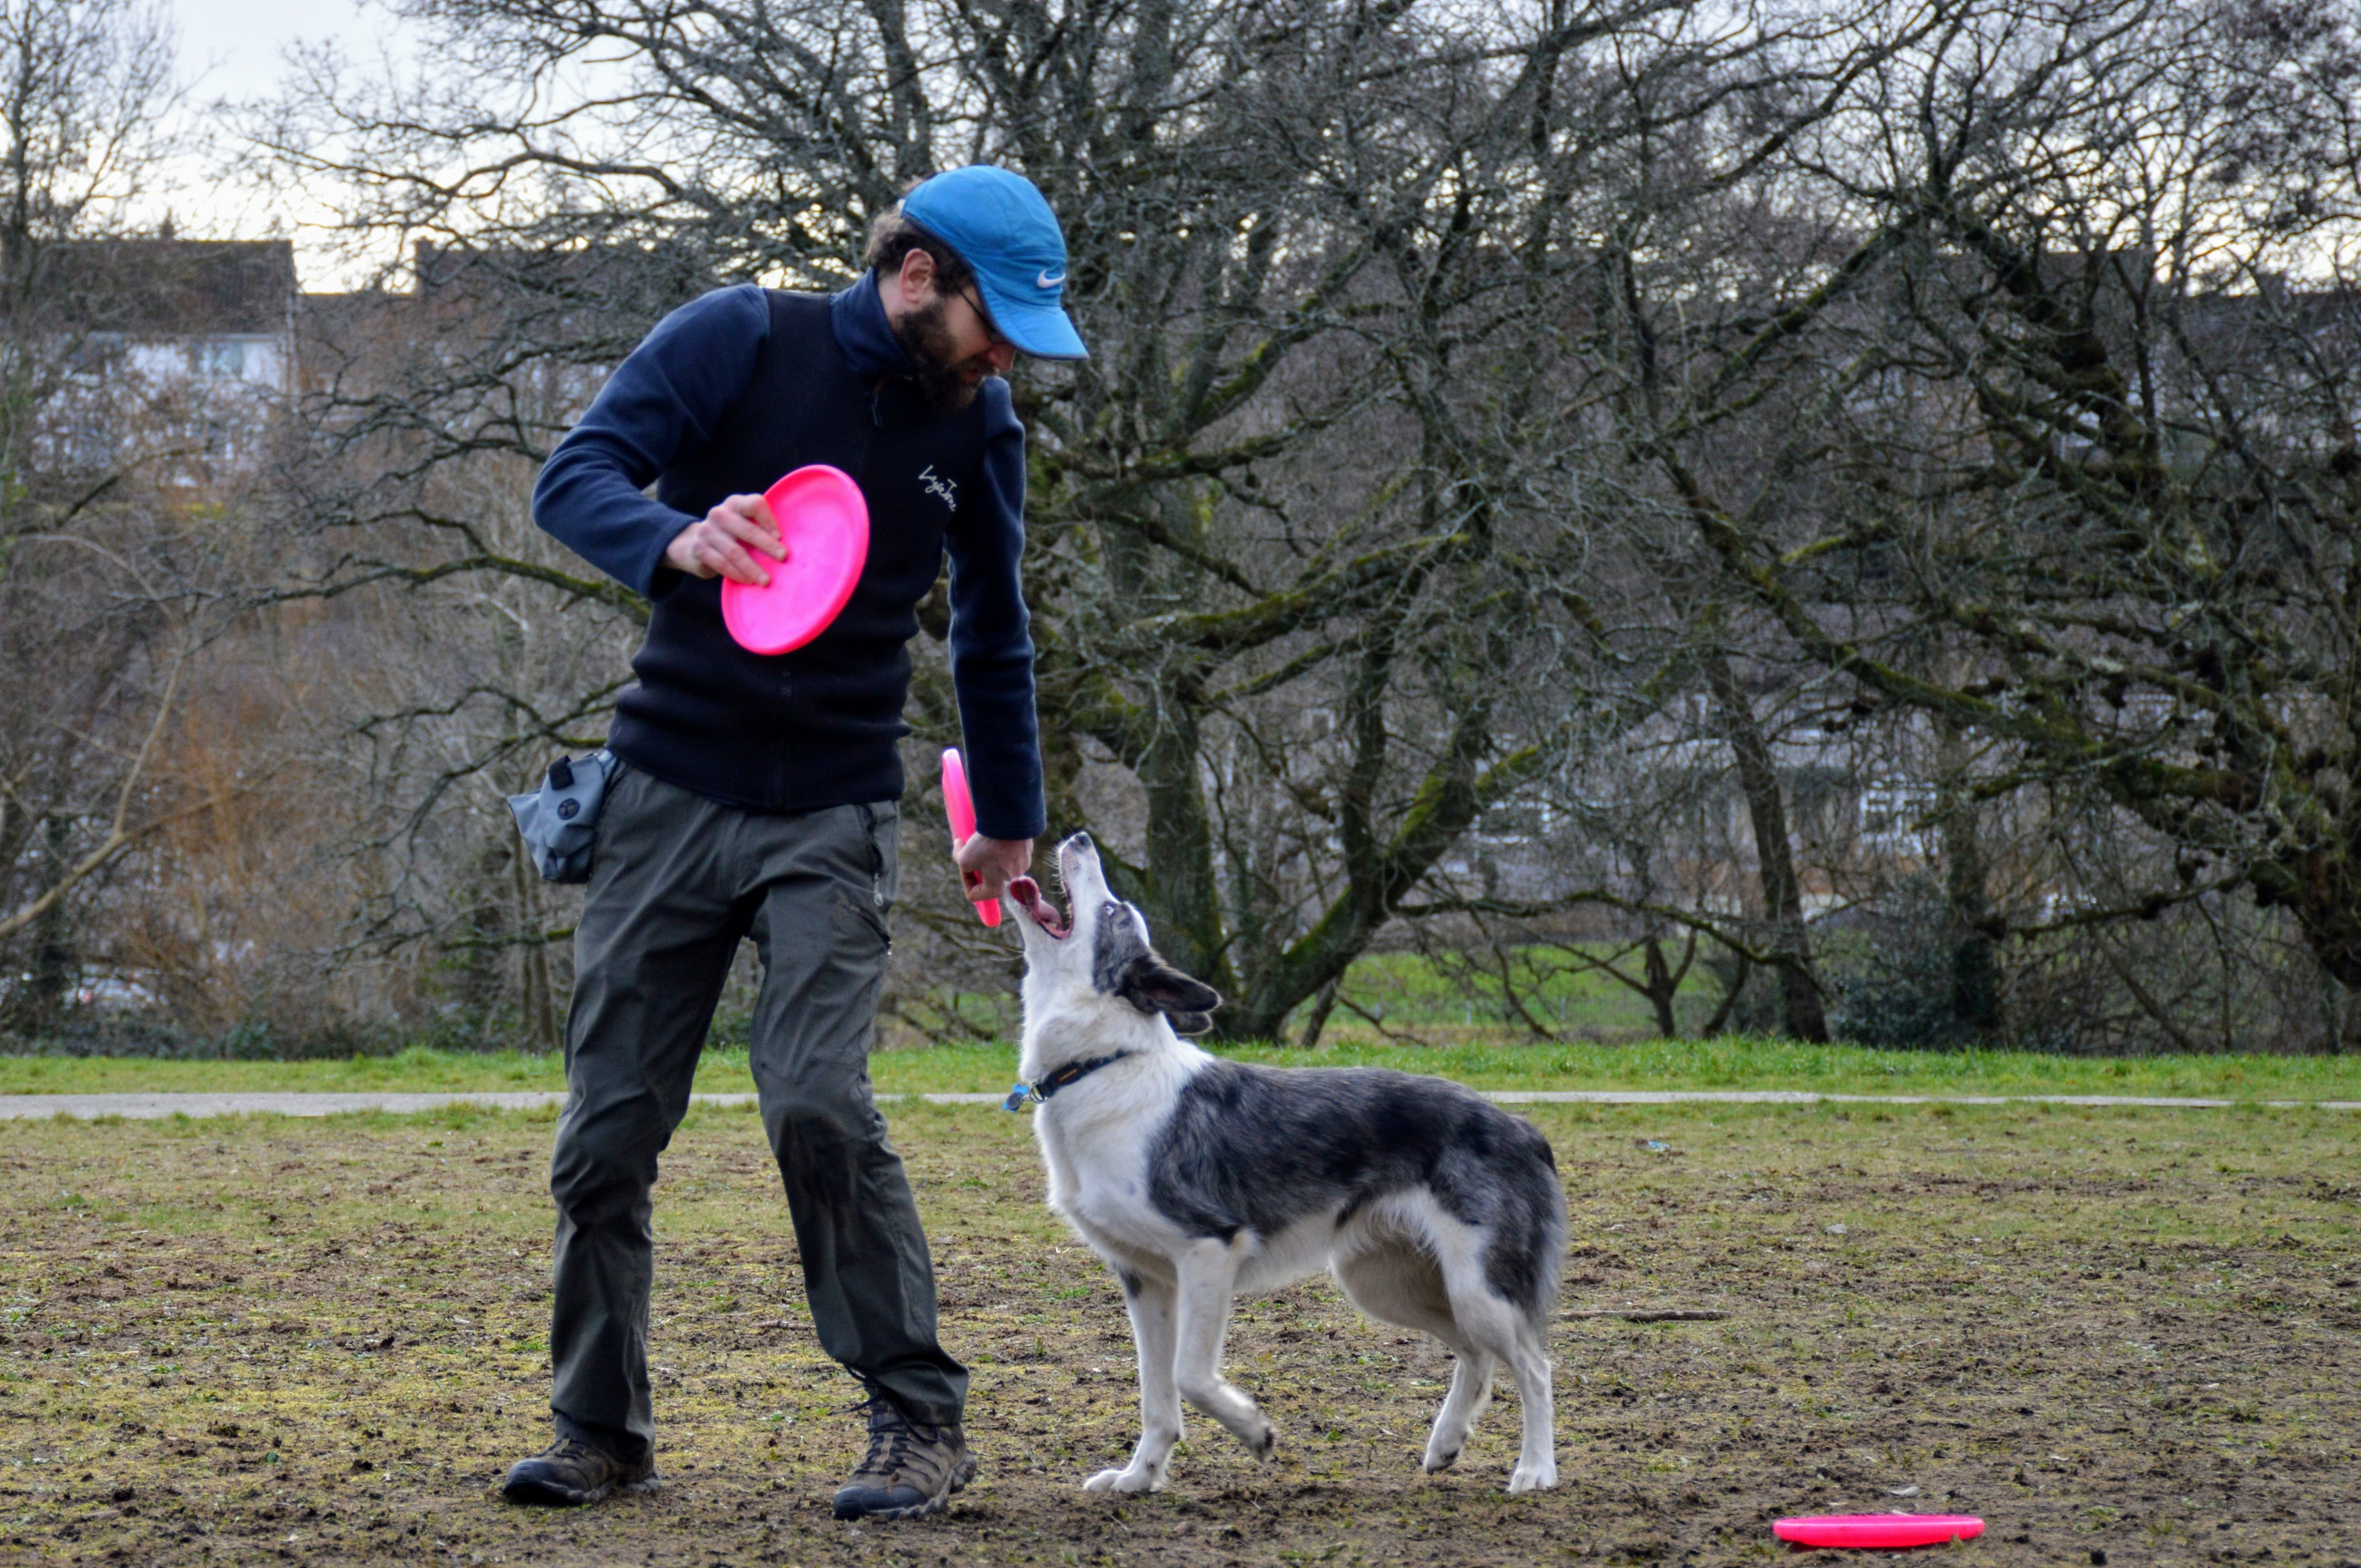
\includegraphics[width=.45\textwidth]{pup_4.jpg}
    \end{center}

}

\frame{
    \Large
    \begin{quote}
        ``4-5 lecture slot is a pain!''
    \end{quote}
}

\frame{
    \Large
    \begin{quote}
        ``Not sure if problem sheet questions are representative of exam style
        questions?''
    \end{quote}
}

\frame{
    \Large
    \begin{quote}
        ``Printing mishaps (sorry)''
    \end{quote}
}


\frame{
    \Large
    \begin{quote}
        ``It would be nice if sometime the professor told us how to write the
        code''
    \end{quote}
}

\frame{
    \begin{quote}
        ``Code provided in alternative languages e.g. R would be nice.''
    \end{quote}
}

\frame{
    \Large
    \begin{quote}
        ``More explanation in the sheet solutions''
    \end{quote}
}

\frame{
    \Large
    \begin{quote}
        ``Coursework page limit! There is a lot that I would to have been able
        to include in the report! (At least 3 pages please)''
    \end{quote}
}

\frame{
    \Large
    \begin{quote}
        ``Lectures can be inconsistent in pace and difficulty.''
    \end{quote}
}

\frame{
    \Large
    \begin{quote}
        ``I don't know if you expect this class to be a reversed teaching style or
        not. Are you expecting us to pre-read for lectures? It seems like you
        like us to `discover' stuff in class.''
    \end{quote}
}

\frame{
    \Large
    \begin{quote}
        ```Class meeting' is a funny term for lecture.''
    \end{quote}
}

\frame{
    \Large
    \begin{quote}
        The room is not appropriate.
    \end{quote}
}

\frame{
    \Large
    \begin{quote}
        ``Perhaps go through big topics a little more slowly (eg how you went
        through Best Response Polytopes over two lectures).''
    \end{quote}
}

\frame{
    \Large
    \begin{quote}
        ``Sometimes I feel like you get angry when we don't understand
        something''
    \end{quote}
}

\frame{
    \Large
    \begin{quote}
        ``More guidance on coursework!''
    \end{quote}
}

\frame{
    \Large
    \begin{quote}
        ``Impact of not starting on time but waiting for people to be quiet
        impacts everyone, not just the people talking.''
    \end{quote}
}

\frame{
    \Large
    \begin{quote}
        ``Not enough cake (ie not every lecture)''
    \end{quote}
}

\frame{
    \Large
    \begin{quote}
        ``I like the beard''
    \end{quote}
}


\end{document}
